\documentclass[11pt, a4paper]{article}
\usepackage{xparse}
\usepackage{pgfplots}
\pgfplotsset{compat=1.18}
\usepackage{subcaption}
\usepackage[textwidth=4.8041in]{geometry}

\usepgfplotslibrary{external}
\tikzexternalize

\ExplSyntaxOn

\NewDocumentCommand{\getenv}{om}
 {
  \sys_get_shell:nnN { kpsewhich ~ --var-value ~ #2 } { } \l_tmpa_tl
  \tl_trim_spaces:N \l_tmpa_tl
  \IfNoValueTF { #1 }
   {
    \tl_use:N \l_tmpa_tl
   }
   {
    \tl_set_eq:NN #1 \l_tmpa_tl
   }
 }

\ExplSyntaxOff

\getenv[\STAGEOUTPUTPATH]{STAGE_OUTPUT_PATH}

\newcommand{\textsize}{\tiny}

\begin{document}

\begin{figure}
    \centering
    \begin{subfigure}[b]{0.23\textwidth}
        \centering
        \begin{tikzpicture}
            \begin{axis}[
                xlabel={Cover Size},
                ylabel={Correlation},
                colormap name=viridis,
                axis on top,  % ticks on top of matrix
                scale only axis=true,
                width=0.83125\textwidth,
                height=0.83125\textwidth,
                enlarge x limits={abs=0.5},
                enlarge y limits={abs=0.01},
                view={0}{90},
                xticklabel style={font=\textsize, yshift=0.5ex},
                yticklabel style={font=\textsize, xshift=0.5ex},
                label style={font=\textsize},
                xlabel style={yshift=1ex},
                ylabel style={yshift=-1ex},
            ]
                \addplot3 [
                    surf,
                    point meta=explicit,
                    mesh/rows=99,
                    shader=flat corner,
                ] table [x=size, y=correlation, z expr=0, meta=score, col sep=comma] {\STAGEOUTPUTPATH/result_factors_analytical_size_average_ranking_loss_maximal_s0_cb0.csv};

                \addplot3 [
                    contour lua={
                        labels=false,
                        draw color=white,
                    },
                    mesh/rows=99,
                    mesh/cols=100,
                    z filter/.expression={1},
                ] table [
                    x=size, 
                    y=correlation, 
                    z=score, 
                    col sep=comma,
                ] {\STAGEOUTPUTPATH/result_factors_analytical_size_average_ranking_loss_maximal_s0_cb0_smooth.csv};
            \end{axis}
        \end{tikzpicture}
        \caption{
            $\varphi^{rasl}_{0, 0}$
        }
        \label{fig:arl_size_dependency}
    \end{subfigure}
    \begin{subfigure}[b]{0.2\textwidth}
        \centering
        \begin{tikzpicture}
            \begin{axis}[
                xlabel={Cover Size},
                colormap name=viridis,
                axis on top,  % ticks on top of matrix
                scale only axis=true,
                width=0.95\textwidth,
                height=0.95\textwidth,
                enlarge x limits={abs=0.5},
                enlarge y limits={abs=0.01},
                view={0}{90},
                xticklabel style={font=\textsize, yshift=0.5ex},
                label style={font=\textsize},
                xlabel style={yshift=1ex},
                yticklabels={},
            ]
                \addplot3 [
                    surf,
                    point meta=explicit,
                    mesh/rows=99,
                    shader=flat corner,
                ] table [x=size, y=correlation, z expr=0, meta=score, col sep=comma] {\STAGEOUTPUTPATH/result_factors_analytical_size_average_ranking_loss_maximal_s1_cb0.csv};

                \addplot3 [
                    contour lua={
                        labels=false,
                        draw color=white,
                    },
                    mesh/rows=99,
                    mesh/cols=100,
                    z filter/.expression={1},
                ] table [
                    x=size, 
                    y=correlation, 
                    z=score, 
                    col sep=comma,
                ] {\STAGEOUTPUTPATH/result_factors_analytical_size_average_ranking_loss_maximal_s1_cb0_smooth.csv};
            \end{axis}
        \end{tikzpicture}
        \caption{
            $\varphi^{rasl}_{1, 0}$
        }
        \label{fig:arl_weighted_size_dependency}
    \end{subfigure}
    \begin{subfigure}[b]{0.23\textwidth}
        \centering
        \begin{tikzpicture}
            \begin{axis}[
                xlabel={NCR},
                ylabel={Correlation},
                colormap name=viridis,
                axis on top,  % ticks on top of matrix
                scale only axis=true,
                width=0.83125\textwidth,
                height=0.83125\textwidth,
                enlarge x limits={abs=0.005},
                enlarge y limits={abs=0.01},
                view={0}{90},
                xticklabel style={font=\textsize, yshift=0.5ex},
                yticklabel style={font=\textsize, xshift=0.5ex},
                label style={font=\textsize},
                xlabel style={yshift=1ex},
                ylabel style={yshift=-1ex},
                xtick={0.25,0.5,0.75,1.0},
            ]
                \addplot3 [
                    surf,
                    point meta=explicit,
                    mesh/rows=100,
                    shader=flat corner,
                ] table [x=negative_class_ratio, y=correlation, z expr=0, meta=score, col sep=comma] {\STAGEOUTPUTPATH/result_factors_analytical_class_balance_average_ranking_loss_maximal_s0_cb0.csv};

                \addplot3 [
                    contour lua={
                        labels=false,
                        draw color=white,
                    },
                    mesh/rows=100,
                    mesh/cols=100,
                    z filter/.expression={1},
                ] table [
                    x=negative_class_ratio, 
                    y=correlation, 
                    z=score, 
                    col sep=comma,
                ] {\STAGEOUTPUTPATH/result_factors_analytical_class_balance_average_ranking_loss_maximal_s0_cb0_smooth.csv};
            \end{axis}
        \end{tikzpicture}
        \caption{
            $\varphi^{rasl}_{0, 0}$
        }
        \label{fig:arl_class_balance_dependency}
    \end{subfigure}
    \begin{subfigure}[b]{0.2\textwidth}
        \centering
        \begin{tikzpicture}
            \begin{axis}[
                xlabel={NCR},
                colormap name=viridis,
                axis on top,  % ticks on top of matrix
                scale only axis=true,
                width=0.95\textwidth,
                height=0.95\textwidth,
                enlarge x limits={abs=0.005},
                enlarge y limits={abs=0.01},
                view={0}{90},
                xticklabel style={font=\textsize, yshift=0.5ex},
                label style={font=\textsize},
                xlabel style={yshift=1ex},
                yticklabels={},
                xtick={0.25,0.5,0.75,1.0},
            ]
                \addplot3 [
                    surf,
                    point meta=explicit,
                    mesh/rows=100,
                    shader=flat corner,
                ] table [x=negative_class_ratio, y=correlation, z expr=0, meta=score, col sep=comma] {\STAGEOUTPUTPATH/result_factors_analytical_class_balance_average_ranking_loss_maximal_s0_cb1.csv};

                \addplot3 [
                    contour lua={
                        labels=false,
                        draw color=white,
                    },
                    mesh/rows=100,
                    mesh/cols=100,
                    z filter/.expression={1},
                ] table [
                    x=negative_class_ratio, 
                    y=correlation, 
                    z=score, 
                    col sep=comma,
                ] {\STAGEOUTPUTPATH/result_factors_analytical_class_balance_average_ranking_loss_maximal_s0_cb1_smooth.csv};
            \end{axis}
        \end{tikzpicture}
        \caption{
            $\varphi^{rasl}_{0, 1}$
        }
        \label{fig:arl_weighted_class_balance_dependency}
    \end{subfigure}
    \\
    \begin{subfigure}[b]{0.23\textwidth}
        \centering
        \begin{tikzpicture}
            \begin{axis}[
                xlabel={Cover Size},
                ylabel={Correlation},
                colormap name=viridis,
                axis on top,  % ticks on top of matrix
                scale only axis=true,
                width=0.83125\textwidth,
                height=0.83125\textwidth,
                enlarge x limits={abs=0.5},
                enlarge y limits={abs=0.01},
                view={0}{90},
                xticklabel style={font=\textsize, yshift=0.5ex},
                yticklabel style={font=\textsize, xshift=0.5ex},
                label style={font=\textsize},
                xlabel style={yshift=1ex},
                ylabel style={yshift=-1ex},
            ]
                \addplot3 [
                    surf,
                    point meta=explicit,
                    mesh/rows=99,
                    shader=flat corner,
                ] table [x=size, y=correlation, z expr=0, meta=score, col sep=comma] {\STAGEOUTPUTPATH/result_factors_analytical_size_roc_auc_score_maximal_s0_cb0.csv};

                \addplot3 [
                    contour lua={
                        labels=false,
                        draw color=white,
                    },
                    mesh/rows=99,
                    mesh/cols=100,
                    z filter/.expression={1},
                ] table [
                    x=size, 
                    y=correlation, 
                    z=score, 
                    col sep=comma,
                ] {\STAGEOUTPUTPATH/result_factors_analytical_size_roc_auc_score_maximal_s0_cb0_smooth.csv};
            \end{axis}
        \end{tikzpicture}
        \caption{
            $\varphi^{rROCAUC}_{0, 0}$
        }
        \label{fig:roc_auc_size_dependency}
    \end{subfigure}
    \begin{subfigure}[b]{0.2\textwidth}
        \centering
        \begin{tikzpicture}
            \begin{axis}[
                xlabel={Cover Size},
                colormap name=viridis,
                axis on top,  % ticks on top of matrix
                scale only axis=true,
                width=0.95\textwidth,
                height=0.95\textwidth,
                enlarge x limits={abs=0.5},
                enlarge y limits={abs=0.01},
                view={0}{90},
                xticklabel style={font=\textsize, yshift=0.5ex},
                label style={font=\textsize},
                xlabel style={yshift=1ex},
                yticklabels={},
            ]
                \addplot3 [
                    surf,
                    point meta=explicit,
                    mesh/rows=99,
                    shader=flat corner,
                ] table [x=size, y=correlation, z expr=0, meta=score, col sep=comma] {\STAGEOUTPUTPATH/result_factors_analytical_size_roc_auc_score_maximal_s1_cb0.csv};

                \addplot3 [
                    contour lua={
                        labels=false,
                        draw color=white,
                    },
                    mesh/rows=99,
                    mesh/cols=100,
                    z filter/.expression={1},
                ] table [
                    x=size, 
                    y=correlation, 
                    z=score, 
                    col sep=comma,
                ] {\STAGEOUTPUTPATH/result_factors_analytical_size_roc_auc_score_maximal_s1_cb0_smooth.csv};
            \end{axis}
        \end{tikzpicture}
        \caption{
            $\varphi^{rROCAUC}_{1, 0}$
        }
        \label{fig:roc_auc_weighted_size_dependency}
    \end{subfigure}
    \begin{subfigure}[b]{0.23\textwidth}
        \centering
        \begin{tikzpicture}
            \begin{axis}[
                xlabel={NCR},
                ylabel={Correlation},
                colormap name=viridis,
                axis on top,  % ticks on top of matrix
                scale only axis=true,
                width=0.83125\textwidth,
                height=0.83125\textwidth,
                enlarge x limits={abs=0.005},
                enlarge y limits={abs=0.01},
                view={0}{90},
                xticklabel style={font=\textsize, yshift=0.5ex},
                yticklabel style={font=\textsize, xshift=0.5ex},
                label style={font=\textsize},
                xlabel style={yshift=1ex},
                ylabel style={yshift=-1ex},
                xtick={0.25,0.5,0.75,1.0},
            ]
                \addplot3 [
                    surf,
                    point meta=explicit,
                    mesh/rows=100,
                    shader=flat corner,
                ] table [x=negative_class_ratio, y=correlation, z expr=0, meta=score, col sep=comma] {\STAGEOUTPUTPATH/result_factors_analytical_class_balance_roc_auc_score_maximal_s0_cb0.csv};

                \addplot3 [
                    contour lua={
                        labels=false,
                        draw color=white,
                    },
                    mesh/rows=100,
                    mesh/cols=100,
                    z filter/.expression={1},
                ] table [
                    x=negative_class_ratio, 
                    y=correlation, 
                    z=score, 
                    col sep=comma,
                ] {\STAGEOUTPUTPATH/result_factors_analytical_class_balance_roc_auc_score_maximal_s0_cb0_smooth.csv};
            \end{axis}
        \end{tikzpicture}
        \caption{
            $\varphi^{rROCAUC}_{0, 0}$
        }
        \label{fig:roc_auc_class_balance_dependency}
    \end{subfigure}
    \begin{subfigure}[b]{0.2\textwidth}
        \centering
        \begin{tikzpicture}
            \begin{axis}[
                xlabel={NCR},
                colormap name=viridis,
                axis on top,  % ticks on top of matrix
                scale only axis=true,
                width=0.95\textwidth,
                height=0.95\textwidth,
                enlarge x limits={abs=0.005},
                enlarge y limits={abs=0.01},
                view={0}{90},
                xticklabel style={font=\textsize, yshift=0.5ex},
                label style={font=\textsize},
                xlabel style={yshift=1ex},
                yticklabels={},
                xtick={0.25,0.5,0.75,1.0},
            ]
                \addplot3 [
                    surf,
                    point meta=explicit,
                    mesh/rows=100,
                    shader=flat corner,
                ] table [x=negative_class_ratio, y=correlation, z expr=0, meta=score, col sep=comma] {\STAGEOUTPUTPATH/result_factors_analytical_class_balance_roc_auc_score_maximal_s0_cb1.csv};

                \addplot3 [
                    contour lua={
                        labels=false,
                        draw color=white,
                    },
                    mesh/rows=100,
                    mesh/cols=100,
                    z filter/.expression={1},
                ] table [
                    x=negative_class_ratio, 
                    y=correlation, 
                    z=score, 
                    col sep=comma,
                ] {\STAGEOUTPUTPATH/result_factors_analytical_class_balance_roc_auc_score_maximal_s0_cb1_smooth.csv};
            \end{axis}
        \end{tikzpicture}
        \caption{
            $\varphi^{rROCAUC}_{0, 1}$
        }
        \label{fig:roc_auc_weighted_class_balance_dependency}
    \end{subfigure}
    \\
    \begin{subfigure}[b]{0.23\textwidth}
        \centering
        \begin{tikzpicture}
            \begin{axis}[
                xlabel={Cover Size},
                ylabel={Correlation},
                colormap name=viridis,
                axis on top,  % ticks on top of matrix
                scale only axis=true,
                width=0.83125\textwidth,
                height=0.83125\textwidth,
                enlarge x limits={abs=0.5},
                enlarge y limits={abs=0.01},
                view={0}{90},
                xticklabel style={font=\textsize, yshift=0.5ex},
                yticklabel style={font=\textsize, xshift=0.5ex},
                label style={font=\textsize},
                xlabel style={yshift=1ex},
                ylabel style={yshift=-1ex},
            ]
                \addplot3 [
                    surf,
                    point meta=explicit,
                    mesh/rows=99,
                    shader=flat corner,
                ] table [x=size, y=correlation, z expr=0, meta=score, col sep=comma] {\STAGEOUTPUTPATH/result_factors_analytical_size_prc_auc_score_maximal_s0_cb0.csv};

                \addplot3 [
                    contour lua={
                        labels=false,
                        draw color=white,
                    },
                    mesh/rows=99,
                    mesh/cols=100,
                    z filter/.expression={1},
                ] table [
                    x=size, 
                    y=correlation, 
                    z=score, 
                    col sep=comma,
                ] {\STAGEOUTPUTPATH/result_factors_analytical_size_prc_auc_score_maximal_s0_cb0_smooth.csv};
            \end{axis}
        \end{tikzpicture}
        \caption{
            $\varphi^{rPRAUC}_{0, 0}$
        }
        \label{fig:pr_auc_size_dependency}
    \end{subfigure}
    \begin{subfigure}[b]{0.2\textwidth}
        \centering
        \begin{tikzpicture}
            \begin{axis}[
                xlabel={Cover Size},
                colormap name=viridis,
                axis on top,  % ticks on top of matrix
                scale only axis=true,
                width=0.95\textwidth,
                height=0.95\textwidth,
                enlarge x limits={abs=0.5},
                enlarge y limits={abs=0.01},
                view={0}{90},
                xticklabel style={font=\textsize, yshift=0.5ex},
                label style={font=\textsize},
                xlabel style={yshift=1ex},
                yticklabels={},
            ]
                \addplot3 [
                    surf,
                    point meta=explicit,
                    mesh/rows=99,
                    shader=flat corner,
                ] table [x=size, y=correlation, z expr=0, meta=score, col sep=comma] {\STAGEOUTPUTPATH/result_factors_analytical_size_prc_auc_score_maximal_s1_cb0.csv};

                \addplot3 [
                    contour lua={
                        labels=false,
                        draw color=white,
                    },
                    mesh/rows=99,
                    mesh/cols=100,
                    z filter/.expression={1},
                ] table [
                    x=size, 
                    y=correlation, 
                    z=score, 
                    col sep=comma,
                ] {\STAGEOUTPUTPATH/result_factors_analytical_size_prc_auc_score_maximal_s1_cb0_smooth.csv};
            \end{axis}
        \end{tikzpicture}
        \caption{
            $\varphi^{rPRAUC}_{1, 0}$
        }
        \label{fig:pr_auc_weighted_size_dependency}
    \end{subfigure}
    \begin{subfigure}[b]{0.23\textwidth}
        \centering
        \begin{tikzpicture}
            \begin{axis}[
                xlabel={NCR},
                ylabel={Correlation},
                colormap name=viridis,
                axis on top,  % ticks on top of matrix
                scale only axis=true,
                width=0.83125\textwidth,
                height=0.83125\textwidth,
                enlarge x limits={abs=0.005},
                enlarge y limits={abs=0.01},
                view={0}{90},
                xticklabel style={font=\textsize, yshift=0.5ex},
                yticklabel style={font=\textsize, xshift=0.5ex},
                label style={font=\textsize},
                xlabel style={yshift=1ex},
                ylabel style={yshift=-1ex},
                xtick={0.25,0.5,0.75,1.0},
            ]
                \addplot3 [
                    surf,
                    point meta=explicit,
                    mesh/rows=100,
                    shader=flat corner,
                ] table [x=negative_class_ratio, y=correlation, z expr=0, meta=score, col sep=comma] {\STAGEOUTPUTPATH/result_factors_analytical_class_balance_prc_auc_score_maximal_s0_cb0.csv};

                \addplot3 [
                    contour lua={
                        labels=false,
                        draw color=white,
                    },
                    mesh/rows=100,
                    mesh/cols=100,
                    z filter/.expression={1},
                ] table [
                    x=negative_class_ratio, 
                    y=correlation, 
                    z=score, 
                    col sep=comma,
                ] {\STAGEOUTPUTPATH/result_factors_analytical_class_balance_prc_auc_score_maximal_s0_cb0_smooth.csv};
            \end{axis}
        \end{tikzpicture}
        \caption{
            $\varphi^{rPRAUC}_{0, 0}$
        }
        \label{fig:pr_auc_class_balance_dependency}
    \end{subfigure}
    \begin{subfigure}[b]{0.2\textwidth}
        \centering
        \begin{tikzpicture}
            \begin{axis}[
                xlabel={NCR},
                colormap name=viridis,
                axis on top,  % ticks on top of matrix
                scale only axis=true,
                width=0.95\textwidth,
                height=0.95\textwidth,
                enlarge x limits={abs=0.005},
                enlarge y limits={abs=0.01},
                view={0}{90},
                xticklabel style={font=\textsize, yshift=0.5ex},
                label style={font=\textsize},
                xlabel style={yshift=1ex},
                yticklabels={},
                xtick={0.25,0.5,0.75,1.0},
            ]
                \addplot3 [
                    surf,
                    point meta=explicit,
                    mesh/rows=100,
                    shader=flat corner,
                ] table [x=negative_class_ratio, y=correlation, z expr=0, meta=score, col sep=comma] {\STAGEOUTPUTPATH/result_factors_analytical_class_balance_prc_auc_score_maximal_s0_cb1.csv};

                \addplot3 [
                    contour lua={
                        labels=false,
                        draw color=white,
                    },
                    mesh/rows=100,
                    mesh/cols=100,
                    z filter/.expression={1},
                ] table [
                    x=negative_class_ratio, 
                    y=correlation, 
                    z=score, 
                    col sep=comma,
                ] {\STAGEOUTPUTPATH/result_factors_analytical_class_balance_prc_auc_score_maximal_s0_cb1_smooth.csv};
            \end{axis}
        \end{tikzpicture}
        \caption{
            $\varphi^{rPRAUC}_{0, 1}$
        }
        \label{fig:pr_auc_weighted_class_balance_dependency}
    \end{subfigure}
\end{figure}

\begin{figure}
    \begin{subfigure}{\textwidth}
        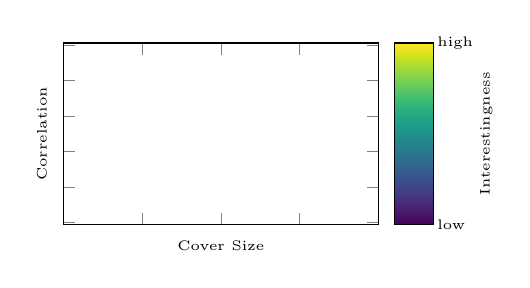
\begin{tikzpicture}
            \begin{axis}[
                xlabel={Cover Size},
                ylabel={Correlation},
                colorbar,
                colorbar style={
                    ylabel=Interestingness,
                    yticklabel style={font=\textsize, xshift=-0.5ex},
                    label style={font=\textsize},
                    ylabel style={yshift=1ex},
                    ytick={0,1},
                    yticklabels={low, high},
                    at={(1.05,1)},
                },
                colormap name=viridis,
                point meta min=0,
                point meta max=1,
                axis on top,  % ticks on top of matrix
                scale only axis=true,
                width=0.33\textwidth,
                height=0.19\textwidth,
                enlarge x limits={abs=0.5},
                enlarge y limits={abs=0.01},
                view={0}{90},
                yticklabels={},
                xticklabels={},
                label style={font=\textsize},
                xlabel style={yshift=1ex},
                ylabel style={yshift=-1ex},
            ]
            
            \end{axis}
        \end{tikzpicture}
    \end{subfigure}
\end{figure}

\end{document}
